%% \section{The blinkered policy}

%% \section{The blinkered policy}

%% This is the key section.  Write it, and then see what prereqs are required.

The myopic policy is an extreme approximation, often stopping far too early.
A better approximation can be obtained, at least for the case where
each computation can only affect the value of one action.
The technical definition (closely related to {\em subtree independence} in 
Russell and Wefald's work) is as follows:

\begin{dfn}\label{dfn:independent-actions}
	A metalevel probability model $(U_1,\dots,U_k,\Evidence)$ 
	has \term{independent actions} if the computational variables can be partitioned 
	$\Evidence = \Evidence_1\cup\dots\cup\Evidence_k$ such that such that
	the sets $\{U_i\}\cup\Evidence_i$ are independent of each other for different $i$.	
\end{dfn}

With independent actions, we can talk about metalevel policies that focus on
computations affecting a single action. These policies are not myopic---they can consider arbitrarily many computations---but they are {\em blinkered} because they can look
in only a single direction at a time:

\begin{dfn}\label{dfn:blinkered}
	Given a metalevel decision problem $M=(S,s_0,A_s,T,R)$ with independent actions,
	the \term{blinkered policy} $\pi^b$ is defined by $\pi^b(s) = \argmax_{a\in A_s} Q^b(s,a)$ where
	$Q^b(s,\bot) = \bot$ and for $E_i\in\Evidence_i$
	\begin{equation}\label{eq:blinkered}
		Q^b(s,E_i) = \sup_{\pi\in\Pi^b_i} Q^\pi(s,E_i)
	\end{equation}
	where $\Pi^b_i$ is the set of policies $\pi$ where $\pi(s)\in\Evidence_i$ for all $s\in S$.
\end{dfn}

Clearly, blinkered policies are better than myopic: $Q^m(s,a) \le Q^b(s,a) \le Q^*(s,a)$.
Moreover, the blinkered policy can be computed in time proportional to the number of arms, by breaking the
decision problem into separate subproblems:

\begin{dfn}\label{dfn:one-action}
	Given a metalevel decision problem $M=(S,s_0,A_s,T,R)$ with independent actions,
	a \term{one-action metalevel decision problem} for $i=1,\dots,k$ is the metalevel decision
	problem $M^1_{i,\lambda} = (S_i,s_0,A_{s0},T_i,R_i)$ defined by the metalevel probability
	model $(U_0,U_i,\Evidence_i)$ with $U_0=\lambda$.
\end{dfn}

Note that given a state $s$ of a metalevel decision problem, we can form a state
$s_i$ by taking only the results of computations in $\Evidence_i$ (see \dfnref{dfn:metalevel-mdp}).
By action independence, $\mu_i(s)$ is a function only of $s_i$.

\begin{thm}\label{thm:blinkered}
Given a metalevel decision problem $M=(S,s_0,A_s,T,R)$ with independent actions,
let $M^1_{i,\lambda_i}$ be the $i$th one-action metalevel decision problem for $i=1,\dots,k$.
Then for any $s\in S$, whenever $E_i\in A_s\cap\Evidence_i$ we have:
\[
	Q^b_M(s,E_i) = Q^*_{M^1_{i,\mu^*_{-i}}}(s_i, E_i)
\]
where $\mu^*_{-i} = \max_{j\neq i} \mu_j(s)$.
\end{thm}

\begin{hiddenproof}
	\begin{proof}
	Fix a state $s$, a $E_i\in A_s$ and take any $\pi\in\Pi^b_i$.  Note that such policies
	are equivalent to polices $\pi'$ on $M^1_{1,m}$, and all such policies are represented.
	Consider $Q^\pi(s,E_i)$.  As $\pi(s)\in\Evidence_i$ for all $s\in S$, by action independence $\mu_j(S_n) = \mu_j(s)$.
	By this and \thmref{thm:value-of-computation}, then,
	\[
		Q^\pi_M(s,E_i) = \IE^\pi_M[ -c\,N + \max(\mu_i(S_N), m_i) \given S_0=s, A_0=E_i].
	\]
	Noting that $\mu_i(S_N)$ is a function only of $(S_N)_i$, and that since 
	But then this is exactly $Q^*_{M^1_{i,\mu^*_{-i}}}(s_i, E_i)$.  Taking the supremum
	over $\pi$ gives the result.
	\end{proof}	
\end{hiddenproof}

\thmref{thm:blinkered} shows that to compute the blinkered policy we need
only compute the optimal policies for $k$ separate one-action problems.

For the Bernoulli problem with $k$ actions, the one-action metalevel decision problems
are all one-action Bernoulli problems (\exampleref{example:bernoulli}).  By \thmref{thm:one-action-bound}
these policies perform at most $1/4c - 3$ computations.
As a result, the blinkered policy can be numerically computed in time $O(D/c^2)$ 
independent of $k$ by backwards induction, where $D$ is the number of points $\lambda\in[0,1]$
for which we compute $Q^*_{M^1_{i,m}}(s)$.\footnote{in our experiments below, $D=129$ points are equally spaced,
using linear interpolation between points.}  This will be worth the cost in 
the same situations as mentioned at the end of \secref{sec:optimal}.

\figref{fig:blinkered} compares the blinkered policy 
to several other policies from the literature, using a
Bernoulli sampling problem with $k=25$ and a wide range of values for the step cost $c$.
Performance is measured by expected {\em regret}, where the regret includes the cost of sampling:
$R = (\max_i U_i) - U_j + c\,n$
where $n$ is the number of computations and $j$ is the action actually selected.
The blinkered policy significantly outperforms all others.  The myopic policy
plateaus as it quickly reaches a position where no single computation can
change the final action choice.  ESPb performs quite well given
that is making a normal approximation to the Beta posterior.  
The curves for UCB1-B and UCB1-b show that even given a good stopping rule, UCB1's
choice of actions to sample is not ideal.


\begin{figure}[htb]
\centering
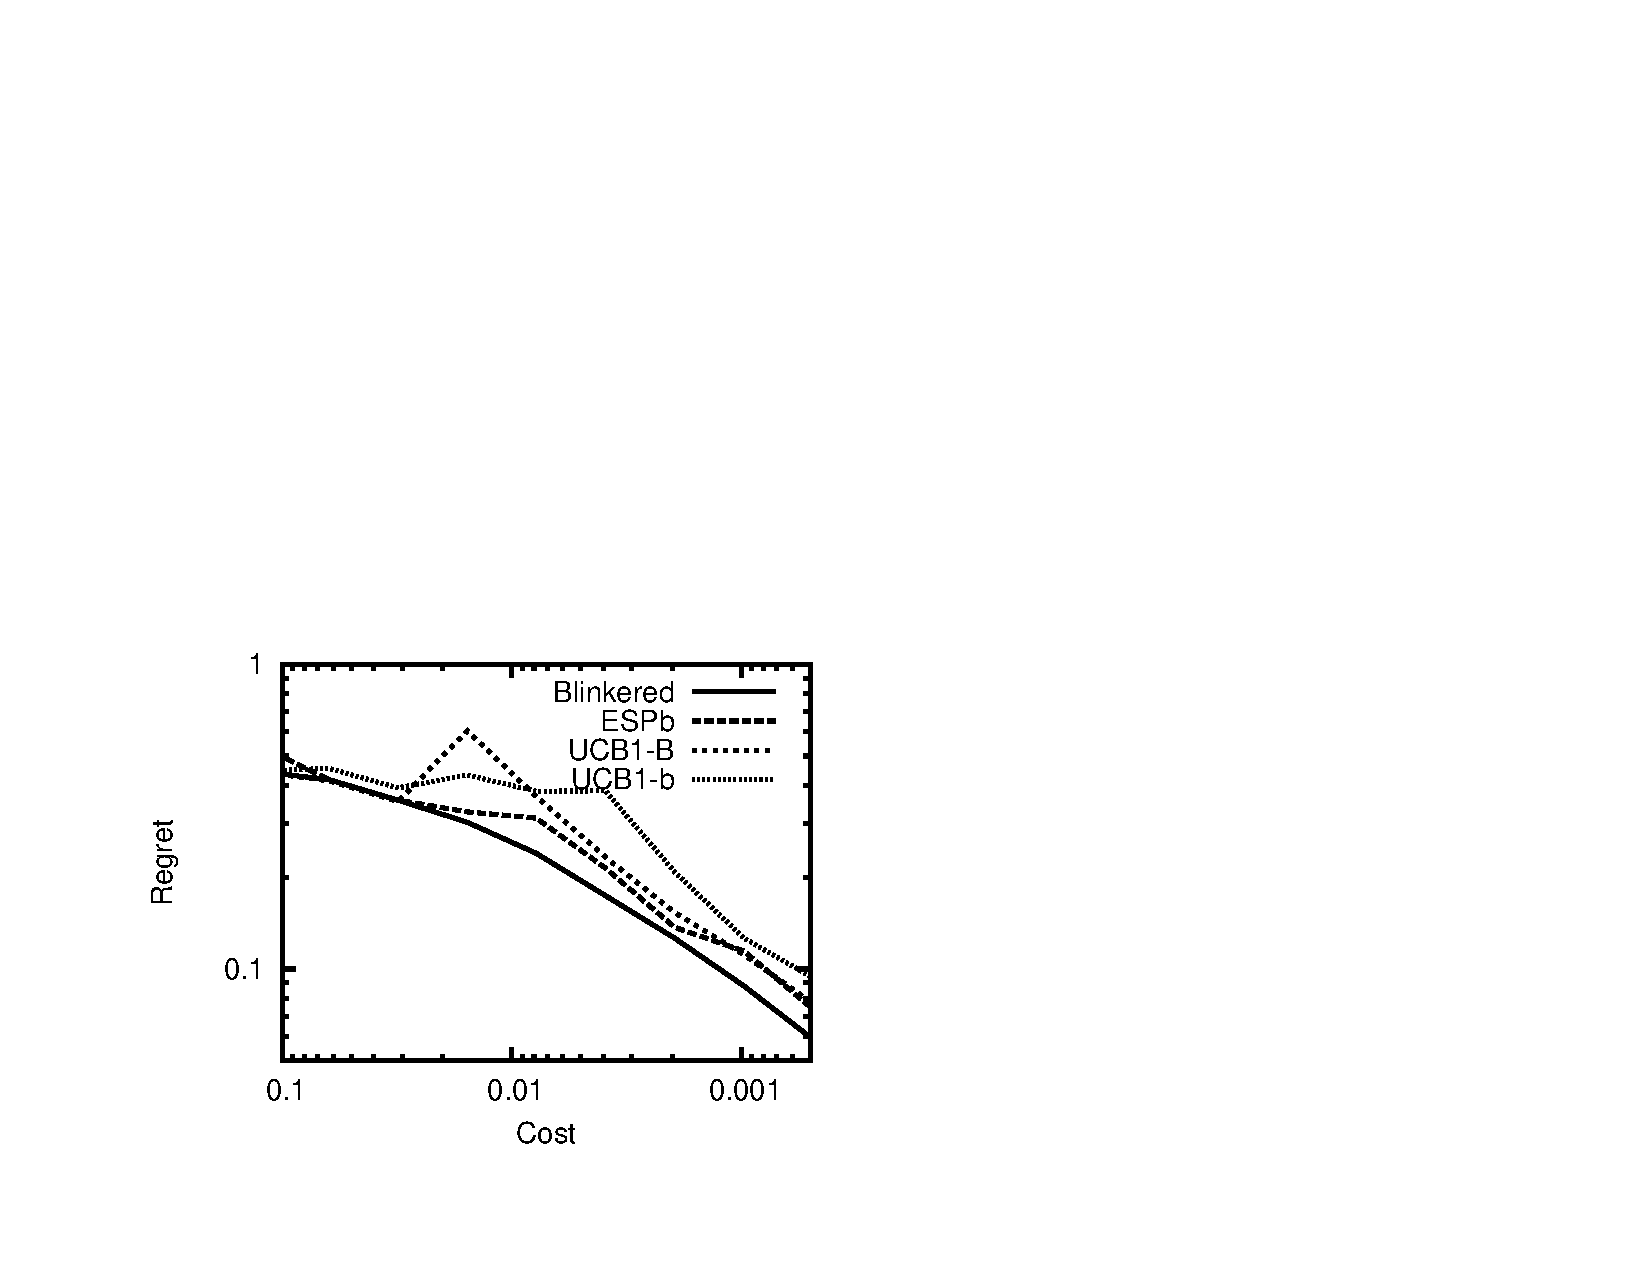
\includegraphics[scale=0.7, trim=90 70 400 300]{blinkered-regret.pdf}
\caption{Average regret of various policies as a function of the cost
in a 25-action Bernoulli sampling problem, over 1000 trials. Error bars
omitted as they are negligible (the relative error is at most 0.03).}
\label{fig:blinkered}
\end{figure}

\begin{comment}
# N: In ~/research/src/mlrl

set terminal postscript enhanced linewidth 2

set size 0.5, 0.5
set logscale xy

set xlabel "Cost"
set ylabel "Samples"
set key left top

set output "blinkered-steps.ps"

plot [0.1:0.00047] "blinkered-steps.dat" title "Blinkered" with lines lw 2, "myopic-steps.dat" title "Myopic" with lines lw 2, "espb-steps.dat" title "ESPb" with lines lw 2, "ucb-blinkered-steps.dat" title "UCB1-B" with lines lw 2, "ucb-blinkered-table-steps.dat" with lines lw 2 title "UCB1-b"

set xlabel "Cost"
set ylabel "Regret"
set key left bottom

set output "blinkered-regret.ps"

plot [0.1:0.00047] [0.05:1] "blinkered-regret.dat" title "Blinkered" with lines lw 2, "myopic-regret.dat" title "Myopic" with lines lw 2, "espb-regret.dat" title "ESPb" with lines lw 2, "ucb-blinkered-regret.dat" title "UCB1-B" with lines lw 2, "ucb-blinkered-table-regret.dat" with lines lw 2 title "UCB1-b"

set output "blinkered-regret-linespoints.ps"

plot [0.1:0.00047] [0.05:1] "blinkered-regret.dat" title "Blinkered" with linespoints lw 2, "myopic-regret.dat" title "Myopic" with linespoints lw 2, "espb-regret.dat" title "ESPb" with linespoints lw 2, "ucb-blinkered-regret.dat" title "UCB1-B" with linespoints lw 2, "ucb-blinkered-table-regret.dat" with linespoints lw 2 title "UCB1-b"

set output "blinkered-regret-errorlines.ps"

plot [0.1:0.00047] [0.05:1] "blinkered-regret2.dat" title "Blinkered" with errorlines lw 2, "myopic-regret2.dat" title "Myopic" with errorlines lw 2, "espb-regret2.dat" title "ESPb" with errorlines lw 2, "ucb-blinkered-regret2.dat" title "UCB1-B" with errorlines lw 2, "ucb-blinkered-table-regret2.dat" with errorlines lw 2 title "UCB1-b"

set output "blinkered-regret-errorlines-nopoints.ps"

plot [0.1:0.00047] [0.05:1] "blinkered-regret.dat" notitle with lines lw 2, "myopic-regret.dat" notitle with lines lw 2, "espb-regret.dat" notitle with lines lw 2, "ucb-blinkered-regret.dat" notitle with lines lw 2, "ucb-blinkered-table-regret.dat" with lines lw 2 notitle, "blinkered-regret2.dat" title "Blinkered" with errorbars lw 2, "myopic-regret2.dat" title "Myopic" with errorbars lw 2, "espb-regret2.dat" title "ESPb" with errorbars lw 2, "ucb-blinkered-regret2.dat" title "UCB1-B" with errorbars lw 2, "ucb-blinkered-table-regret2.dat" with errorlines lw 2 title "UCB1-b"
\end{comment}